\documentclass[]{llncs}   % list options between brackets

\usepackage{color}
\usepackage{graphicx}
\graphicspath{{./figures/}}
\usepackage{subcaption}
%% The amssymb package provides various useful mathematical symbols
\usepackage{amssymb}
\usepackage{standalone}
\usepackage{pgfplots}
%% The amsthm package provides extended theorem environments
%\usepackage{amsthm}
\usepackage{amsmath}
\usepackage{tikz}

\usepackage{listings}

\usepackage{hyperref}

\usepackage{systeme}

\usepackage{enumitem}

\def\shownotes{1}
\def\notesinmargins{0}

\ifnum\shownotes=1
\ifnum\notesinmargins=1
\newcommand{\authnote}[2]{\marginpar{\parbox{\marginparwidth}{\tiny %
  \textsf{#1 {\textcolor{blue}{notes: #2}}}}}%
  \textcolor{blue}{\textbf{\dag}}}
\else
\newcommand{\authnote}[2]{
  \textsf{#1\textcolor{blue}{ #2}}}
\fi
\else
\newcommand{\authnote}[2]{}
\fi

\newcommand{\knote}[1]{{\authnote{\textcolor{green}{Alex notes:}}{#1}}}
\newcommand{\dnote}[1]{{\authnote{\textcolor{red}{Dima notes:}}{#1}}}
\newcommand{\vk}[1]{{\authnote{\textcolor{red}{V:}}{#1}}}

% type user-defined commands here
\usepackage[T1]{fontenc}

\usepackage{xcolor}

\definecolor{dkgreen}{rgb}{0,0.6,0}
\definecolor{gray}{rgb}{0.5,0.5,0.5}
\definecolor{mauve}{rgb}{0.58,0,0.82}

\pgfplotsset{compat=newest, table/search path=figures}

\begin{document}

\title{A Systematic Approach To Cryptocurrency Fees}

%\title{On Space-Scarce Economy\\ In Blockchain Systems}

%\author{Alexander Chepurnoy \and Vasily Kharin \and Dmitry Meshkov}
%\institute{IOHK Research}
\maketitle

\begin{abstract}

%In this paper we study transaction fees in massively replicated open blockchain systems.
%We proposed a new transaction fee scheme based on resources, consumed by the transaction:
%bandwidth, random-access state memory and processor cycles and argue that such a division
%is reasonable based on statistics from Ethereum network.
%The main attention was paid to a component to a transaction fee scheme, which is based on
%how much additional space will be needed for new objects created in result of
%transaction processing and for how long they will live in the state.

In this paper we study transaction fees in massively replicated open
blockchain systems. In these systems, such as Bitcoin, memory to hold a current
state snapshot needed to validate transactions becomes a scarce resource 
eventually. Uncontrolled state size growth could lead
to security issues. 
%The problem is even more critical for blockchain systems used to store data~(such as votes, certificates, logs).
We propose to add a new component to a transaction fee scheme, which is based on
how much additional space will be needed for new objects created in result of
transaction processing and for how long they will live in the state.
We propose how to combine fees charged for different resources spent~(bandwidth, random-access state memory, processor cycles)
in a composite fee and argue that such a separation is reasonable based on statistics from Ethereum network.
We show a possible implementation for charging state-related fee, with regular payments to be charged by miners.

%We provide three possible options towards implementing the new fee component, namely
%\textit{prepaid outputs}, \textit{postpaid outputs} and \textit{scheduled
%payments}. We provide an analysis of the model with respect to all the three
%options.
%\knote{rewrite further} 
% We show that the state growth could be bounded by a fee factor, miners
%are getting additional stable rewards and lost coins are being taken back into
%circulation eventually.    \knote{check this}

\end{abstract}

\section{Introduction}

Bitcoin~\cite{Nakamoto2008} was introduced in 2008 by S. Nakamoto as a purely
peer-to-peer version of electronic cash with a ledger written into blockchain
data structure securely replicated by each network node. Security of the cryptocurrency 
is relied on its mining process. If majority of miners are honest, then Bitcoin
meets its security goals as formal analysis~\cite{Garay2015} shows. For work
done a miner is claiming a reward which consists of two parts. First, some
constant number of bitcoins are created out of thin air according to a
predefined and hard-coded token emission schedule. Second, a miner claims fees
for all the transactions included into the block.

As shown in~\cite{carlsten2016instability} constant block rewards is an important
part of the Bitcoin protocol. Once a predetermined number of coins will enter a circulation
and miners will be rewarded by transaction fees only, their rational behavior will
dramatically differ from the default mining strategy. It is still an open question, whether
Bitcoin will meets its security goals in such circumstances, but at least number of
orphaned blocks will increase making Bitcoin less friendly for regular users.

A transaction fee, which is set by a user during transaction creation, is
useful to limit miners resource usage and prevent spam. In most cases a user pays a fee proportional to transaction size,
limiting miners {\em network} utilization. A rational miner does not
include all the valid transactions into blocks as, due to the increased
chances of orphaning a block, the cost of adding transactions to a block
could not be ignored~\cite{andersen2013,rizun2015transaction}. As shown
in~\cite{rizun2015transaction}, even in absence of block size limit 
Bitcoin fee market is healthy and the miners surplus is maximized at a
finite size of a block. Thus the miner is incentivized to produce
a block of a limited size. Thus only transactions providing enough value to a miner will be included in a block. The 
paper~\cite{rizun2015transaction} provides a procedure to estimate
transaction fee based on block propagation time.

Besides of network utilization, transaction processing requires a miner
to spend some {\em computational} resources.
In Bitcoin the transactional language\cite{script} is very limited, thus
a number of CPU cycles needed to process a transaction
is strictly bounded and corresponding computational costs are not directly
considered. In contrast, in cryptocurrencies supporting smart contract
languages, such as~\cite{seijas2016scripting,tezosScript,solidity},
transaction processing may require a lot of computations, and
corresponding costs are included in transaction fee. Analysis of this fee component is done for concrete systems
in \cite{Earlz2017,luu2015demystifying}, and is out of scope of this paper.

In this work we address a problem of miners {\em storage} resources utilization.
A regular transaction in Bitcoin fully spends outputs from previous transactions, and
also creates new outputs of user-defined values and protecting scripts.
%A notable and the only
%exception is a coinbase transaction of a block which creates fixed amount of
%money out of thin air and also claims transaction fees without referring to any
%outputs~(a fee for a non-coinbase transaction is sum of claimed outputs values
%minus sum of values for created outputs).
A node is checking a transaction in
Bitcoin by using a set of unspent outputs~(UTXO). In other cryptocurrencies a
representation of a {\em state} needed to validate and process an arbitrary
transaction could be different~(for example, in Ethereum~\cite{ethyp} such
structure is called the {\em world state} and fixed by the protocol). To process
a transaction quickly, the state~(or most accessed part of it) should reside in
expensive random-access memory. Once it becomes too big to fit into RAM an attacker can
perform denial-of-service attacks against cryptocurrency nodes. For example,
during attacks on Ethereum in Autumn, 2016, an attacker added about 18 million
accounts to the state~(whose size was less than 1 million accounts before the
attack) and then performed successful denial-of-service attacks against the
nodes~\cite{eth2016dos}. Similarly, in 2013 a denial-of-service attack against
serialized transactions residing in a secondary storage~(HDD or SSD) was
discovered in Bitcoin~\cite{vasek2014empirical}.

In all the cryptocurrencies of today we are aware of, an element of the state once created 
lives possibly forever without paying anything for that. This leads to perpetually increasing state~(we point
to Bitcoin UTXO size as an
example~\cite{utxoChart}). Moreover, state may grow fast during spam attacks, for
example, 15 million outputs were quickly put into UTXO set during spam attacks
against Bitcoin in July 2015~\cite{bitcoin2015flood}, and most of these outputs
are not spent yet. The paper~\cite{reyzin2016improving} is proposing a technical
solution for non-mining nodes where only miners hold the full state~(assuming
that they can invest money in random-access memory of sufficiently big
capacity), while other nodes are checking proofs of state transformations
generated by miners, and size of a proof (in average and also in a worst case)
is about $log(|s|)$ in regards with a state size $|s|$. Nevertheless, big state
could lead to centralization of mining or SPV mining~\cite{spvMining}, and these
concerns should be addressed. The question of internalizing the costs of
state load was raised in~\cite{Moeser2015}, but to the best of our knowledge no
practical solution appeared yet. Also, there is an increasing demand to use a
blockchain as a data storage, and storing permanently objects in the state
without a cleaning procedure is not a viable option.

\subsection{Our contribution}

In this paper we propose an economic solution to the problem of unreasonable state growth
(such as spam attacks, or objects not being using anymore but still living in
the validation state). The solution is a new mandatory fee component. A 
user should pay a fee based on both the additional space needed to store objects
created by a transaction, and also for lifetime of the new bytes. This model is
typical for cloud storage services where users pay for gigabytes of data per
month. 

In the paper we also consider an approach to combine fees charged for different resources consumed by a transaction:
bandwidth, random-access memory to hold state, and processor cycles to process computations prescribed by the transaction.    
We propose to charge only for a resource which consumed at most, so we can say about storage-oriented, network-oriented or computation-oriented transactions. We provide an evaluation of Ethereum usage data which shows that it is possible for this cryptocurrency to determine transaction type.

We propose a convenient way to charge for state memory consumption~(considering output lifetime also). Our approach is convenient for users who often do not know for how long they would like to store their outputs in the system. The approach is called scheduled payments, as we propose to charge periodically for the bytes of memory consumed.



%We provide a possibility for miners to control their storage requirements by changing a fee factor. 
%Later in this paper we will refer to this new fee component as to a {\em space-time fee}.

%Proposed fee regime is promoting money circulation in the blockchain economy.
%The limited lifetime of a state element also leads to lost coins being taken
%back into circulation~(supposedly by miners). 

%Summarizing, we study an economy where quick-access storage of a node in a
%massively-replicated system becomes the most scarce system resource eventually.
%Thus we call such an economy a {\em space-scarce economy}.

\subsection{Structure of the paper}
The paper is organized as follows. We put assumptions behind our model and its analysis into Section~\ref{sec:preliminaries}. Then we provide an algorithm for a composite fee assignment in Section~\ref{sec:algorithm}. We propose a possible approach to charge for state memory consumption in Section~\ref{sec:scheduled}. We show results of Ethereum data evaluation in Section~\ref{sec:evaluation}. We conclude with Section~\ref{sec:conslusion}.

%A design of our new fee component is
%provided in Section~\ref{sec:model}. The model then is analyzed in
%Section~\ref{sec:analysis}. In Section~\ref{sec:rel-work} we observe related
%work, and in Section~\ref{sec:further-work} we shape a plan for further
%research.

\section{Preliminaries}
\label{sec:preliminaries}

We shape our model with the following assumptions:
\begin{enumerate}[label=\textbf{A\arabic*. }]
  % \item All the fees for a block are going to just a miner like in Bitcoin.
  %    There are proposals to share the rewards for a block within a group of
  %    miners, for example in~\cite{eyal2016bitcoin,kogias2016enhancing}, and
  %    they are out of scope of the paper. A notable difference is that if a single miner
  %    is taking all the rewards, he can include his own transactions in it for free
  \item \label{a:utxo} Without loss of generality, we assume throughout the paper that a transaction creates new objects called outputs and spends outputs from previous transactions. Thus the state needed for transaction validation is about a set of outputs yet unspent. The size of the state then is the sum of sizes of all the unspent outputs.  
  \item \label{a:state} We assume that a transaction does not change size of the state significantly
  \item \label{a:miner} For an implementation, we assume that it is profitable for a miner to collect fees from unspent outputs. 
  %\item For simplicity, we assume that a block is of a finite size but all the
  %    transactions a miner has at a moment of block generation can be packed
  %    into it, if otherwise is not stated explicitly
  \item \label{a:minimal} We are considering minimal mandatory fees in the paper. All the nodes
      are checking that a fee paid by a transaction is not less than a minimum
      and rejecting the whole block if it contains a transaction violating fee
      rules. Thus a fee regime is considered as a part of consensus protocol in
      our work. A user can pay more than the minimum to have a higher priority
      for a transaction of interest.
\end{enumerate}


\section{An algorithm for the fee assignment}
\label{sec:algorithm}

As mentioned in the introduction, we develop rules a fee regime having two goals
in mind, namely incentivization of miners and spam prevention.  In this chapter
we reason about the guiding  principles for the fee assignment, and end up with
the example of a practical fee assignment rule.

The evolution of the blockchain networks has demonstrated the main resources
being used. First and the most important so far, the memory of the network nodes 
is limited resource. Blocks in the blockchain after processing are storing on a 
secondary storage, where a cost of a storage unit is low. In contrast, to validate a 
transaction, some state is needed~(for example, unspent outputs set in Bitcoin is used 
to validate a transaction), and this state should reside in expensive random-access memory.   

Second, it becomes obvious, especially with the development of smart contracts,
that a transactional ``cost'' for the node can be more than just a storage:
transactions can contain relatively complicated scripts which are meant to be
executed by all the nodes in the network. The extreme and most famous example is
the Ethereum network implementing the concept of the ``world computer''~\cite{ethyp}. 

Third, there is the network load created by every transaction. If an output is
created in one block and spent right in the next one, it provides almost zero
overhead in terms of validation state size, but creates the network load needed
for synchronization.

A transaction fee should incorporate all the three components stated above.  As
it is demonstrated in~\cite{Earlz2017}, assigning the fee to the storage as if
it was execution of some code can lead to significant disbalance for rich enough
scripting language (for example, for the data being written with an opcode other
than conventional storage one).  Thus, we propose to charge for a component
which demands more resources. That is, storage-oriented transactions should be
charged for state memory consumption, the computation-oriented transactions
should be charged for script execution, and all the others by the network load.
This can be formalized as follows:
\begin{equation}
    \operatorname{Fee}(tx) = \max\left(\alpha \cdot N_b(tx), \beta \cdot N_c(tx),
    S(state) \cdot \sum_i (B_i \cdot L_i) \right)\,.
    \label{eq:max}
\end{equation}
Here $\alpha$ and $\beta$ are the pricing coefficients, $N_b(tx)$ is the number
of bytes in the transaction, which defines the network load, $N_c(tx)$ is the
estimation of the computational cost of transaction, $S(state)$ is the cost of the
storage of byte of output in the state for the unit of time, $L_i$ is the time
for which the output $i$ is being stored in the state, and $B_i$ is its size in
bytes.

Since the time for the data to reside in the state is usually unknown,
the right hand side of Eq.~\eqref{eq:max} cannot be deduced directly at
transaction submission time. For this purpose we introduce a proposal for 
scheduled payments later in Section~\ref{sec:scheduled}. The latter
argument in Eq.~\eqref{eq:max} becomes dominant with time. Starting at the moment $sT$ since transaction when it happens, the
fee is increasing at a constant rate (see Fig.~\ref{fig:max_t}). The possible implementation of this 
algorithm is described in Section~\ref{sec:scheduled}.
\begin{figure}
    \centering
    \begin{subfigure}[b]{.45\textwidth}
    \includestandalone[width=\textwidth]{figures/subsid}
    \caption{Transaction cost as a function of the output existence time.
        \newline
        \label{fig:max_t}}
    \end{subfigure}
    ~
    \begin{subfigure}[b]{.45\textwidth}
        \includestandalone[width=\textwidth]{figures/max_est}
        \caption{Space of transactions split by
            Eq.~\eqref{eq:max} into the subregions of the dominant fees.
            \label{fig:max}}
        \end{subfigure}
        \caption{Fee differentiation by resource consumption}
\end{figure}

The obvious questions here are as follows. What are the guiding principles for
choosing $\alpha$, $\beta$ and $S(\cdot)$? There is also the
question of estimating $N_c(tx)$, which can be solved only by executing the
script for Turing--complete languages. It is known as the worst case execution
time problem~\cite{Wilhelm2008}.  We leave the latter question beyond the scope of
the paper, and answer the former one below.

\subsection{Choice of the relative values of $\alpha$, $\beta$, $S(state)$}

Assume for now, that for every transaction we know for how long the outputs will be
stored in the state. We will overcome this difficulty later. Based on
Eq.~\eqref{eq:max}, we come up with the notion of space of transactions, which
is three--dimensional in our case --- every transaction is defined by three
numbers: $N_b(tx)$, $N_c(tx)$, $N_s(state,tx) = \sum_i (B_i \cdot L_i)$. Eq.~\eqref{eq:max} is splitting 
this space into three regions: network--oriented transactions, space--oriented transactions, 
and computation--oriented transactions (see Figure~\ref{fig:max}). All the splitting 
is governed by the direction of vector $\vec{n}$ which defines the line $\alpha N_b=\beta N_c=N_s$.
Varying the coefficients $\alpha$ and $\beta$, one can change the direction of
$\vec{n}$ adjusting the formal fee prescription to the sensible values.

\subsection{Choice of $S(state)$}

The simplest way of assigning the $S(state)$ value is by making it constant.
%That is, specifying the price of storage of 1 byte of data per one day. 
However, %as it is shown in the Appendix~\ref{apx:statesize} \dnote{do we keep appendix?}, 
this does not fully solve the problem of limiting the state size. What is being controlled in this case,
that is the rate at which the data is being submitted, but not the state size
itself. One could also manually define the maximal size of the state for the
network. This solution, in turn, has its own caveats. For example, once the
state is kept (almost) full by the participants, it can be (almost) impossible
to submit the transaction increasing the state size.  The time till it becomes
possible is hardly predictable. 

Preferable properties of the current state size could be formulated as follows:
it should be predictable, stable, and below some externally given value (an upper
bound on state size, being unique for the whole network). 

Another natural question arising is whether the rigid state size restriction is
necessary?  It is easy to imagine the situation where the formal possibility of
exceeding the state is still present, but hardly ever being used. For example,
if one wants to constrain the state size to 10MB, the possible solution is to
set normal price for submitting data to store if the state size after submission
is below 10MB, but some astronomical price for the luxury of storage above 10MB.
So, formally it will be possible, but in fact, hardly ever used, with every
usage bringing significant profit to miners. The generalization of this idea is
to form the explicit dependence of price on the state load (it will referred to
as ``pricing curve''). The good pricing curve must provide at least one stable
equilibrium of the state size; the minimal dependence on initial conditions (if
possible), and high rewards for miners. The latter could serve as good
optimization parameter. Extreme cases are zero price -- huge data submission --
miners get nothing; and infinite price -- zero data submission -- miners get
nothing. As usual, a maximal outcome is in between.  The pricing policies
described above are two particular cases of pricing curve (see
Figure~\ref{fig:steps}). That is, we assume that the price of data storage in the
state $S(state)$ varies with the current state load $x$. 
\begin{figure} 
    \hfill 
    \begin{tikzpicture} 
        \draw[thick,-stealth] (0,0) -- (0,3) node [right]{$S(state)$}; 
        \draw[thick,-stealth] (0,0) -- (5,0) node [above]{load}; 
        \draw[very thick] (0,0.3) -- (3,0.3) -- (3,3); 
        \draw[dotted] (3,1) -- (3,0) node[below]{$10$MB}; 
    \end{tikzpicture} 
    \hfill 
    \begin{tikzpicture} 
        \draw[thick,-stealth] (0,0) -- (0,3) node [right]{$S(state)$}; 
        \draw[thick,-stealth] (0,0) -- (5,0) node [above]{load}; 
        \draw[very thick] (0,0.3) -- (3,0.3) -- (3,2) -- (5,2); 
        \draw[dotted] (3,1) -- (3,0) node[below]{$10$MB}; 
    \end{tikzpicture} 
    \hfill 
    \caption{ 
        Examples of pricing curves: rigid state size restriction (left) and 
        overflow fees (right, see text). The value of $10$MB is taken 
        arbitrarily.  
    } 
    \label{fig:steps}
\end{figure} 

Note that the pricing curve is defined by a small number of parameters and
to be the same for all the network. To impose an upper bound on the state
size, one can choose the pricing curve formally going to infinity at some finite
state size. The rigid boundary can be provided by divergence higher than
$1/(x_{max}-x)$. One can also try to estimate the optimal state size for a given
differentiable pricing curve. 
%In the continual with the assumptions described in the appendix, 
The data submission rate $N(S(x))$ is fully defined by the
current storage price $S(x)$.  Rewards rate obtained by the miners for stable
state size at price $S$ is given by $y = S \cdot N(S)$. An example is provided in
Figure~\ref{fig:rewards}. First, it provides a possible method of measuring
explicit form of the function $N(S)$ in the model: one has to set up the price,
and observe the static rewards. Second, one may wonder about the price $S^*$,
optimal for the miners in terms of rewards. Obviously, it satisfies
$N(S^*)+S^*N'(S^*)=0$, where prime is derivative with respect to price. As
usual, the optimal price here does not depend on the pricing policy, but rather
the implicit property of the network. \knote{what does the last sentence mean?}  Having the price varying freely can be
considered beneficial both for miners and for network as a whole, since it
allows the first ones to optimize signing strategy, and with this given the
state size is automatically adjusted to the relatively predictable level
$S^{-1}(S^*)$.

\begin{figure}
    \includestandalone[width=\textwidth]{figures/rewards}
    \caption{
        \label{fig:rewards} Example of the rewards curve.
    }
\end{figure}

\section{Scheduled Payments}
\label{sec:scheduled}

In this section we propose a concrete way to charge for state bytes consumed~(or released). There are few possible options for that. A user, for example, may specify lifetime for a coin during its creation and pay for it in advance, this is not very convenient for him though. Another option is to charge when coin is spent, or allow to spend a coin~(by anyone, presumably, a miner) when its value is overweighted by state fee. As a drawback, if coin is associated with a big value, it could live for very long, maybe without a reason. 

We propose more convenient method of charging; we name it {\em scheduled payments}. In this scheme a user must set special predefined script for a coin~(otherwise a transaction and also a block containing it are invalid), which contains a user-specific logic~(we call it {\em regular script}) and a spending condition which allows anyone~(presumably, a miner) to create a transaction claiming this output, necessarily creating a the coin with the same guarding condition and a value not less than original minus a state fee. These two parts~(regular script and a fee charging condition) are connected by using the $\lor$ conjecture. We assume that $\alpha$ and $\beta$ are fixed. We also assume that subsidized period $sT$ \dnote{sT in eq.1 is not a subsidized period! we don not have subsidized period term for now} is to be stored along with the coin by each validating node. Then a guarding script for the coin would be like:

\begin{align}
\begin{split}
&(regular\_script) \lor \\
&(height > (out.height + sT) \land (out.value \le S_c \cdot B \cdot sT \lor \\  
&\qquad tx.has\_output(value = out.value - S_c \cdot B \cdot sT, script = out.script))),
\end{split}
\end{align}
where $height$ is a height of a block which contains a spending transaction, $out.height$ is a height when the output was created, $out.height$ and $out.script$ contain the output's value and spending script respectively, predicate $tx.has\_output()$ checks whether a spending transaction has an output with conditions given as the predicate arguments, and $S_c$ is the value of $S(state)$ when the coin created. As in Section~\ref{sec:algorithm}, constant $B$ is the output size.     


\section{Evaluation}
\label{sec:evaluation}

In this question we experimentally study what could be the real-world
ratio between the pricing coefficients. To extract the realistic possible
values, and verify the validity of described transaction classification, the
data from the Ethereum network was taken. We consider Ethereum a good example,
since all three components of the resource consumption are present in this cryptocurrency. The network load parameter $N_b(tx)$ is simply a transaction size; the state
load $\Delta(tx)$ can be deduced from the blockchain by processing SSTORE
and CREATE operations in transactions. To determine the
computational load $N_c(tx)$, we count Ethereum gas consumed by transaction processing minus its storage cost and
base cost, that is proportional to the transaction size.

\begin{figure}[h]
    \centering
    \begin{subfigure}[b]{0.48\textwidth}
        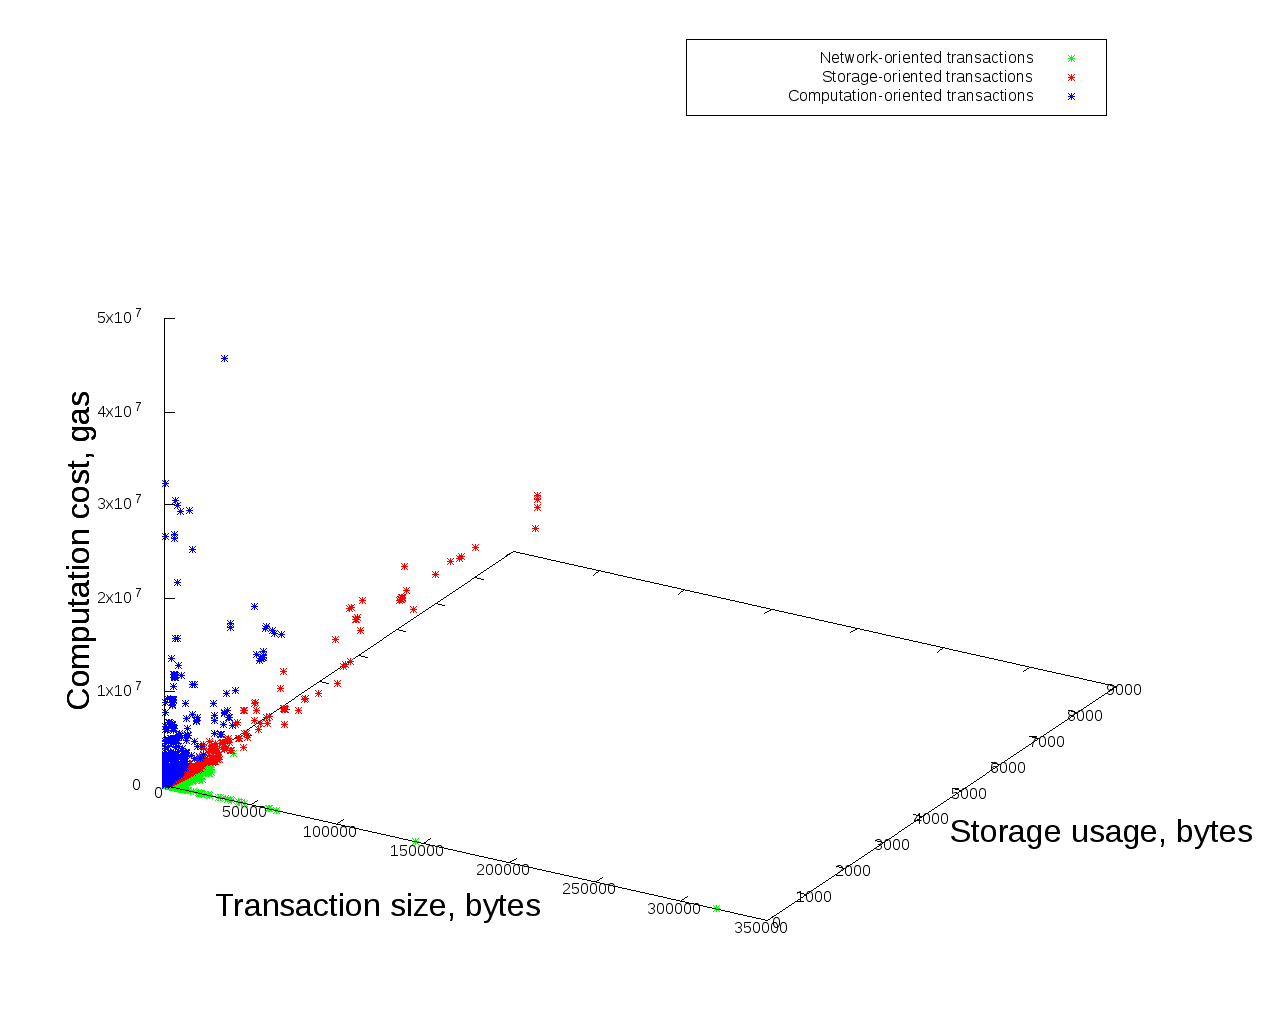
\includegraphics[width=\textwidth]{figures/txs3d}
        \caption{}
        \label{fig:a}
    \end{subfigure}
    \begin{subfigure}[b]{0.48\textwidth}
        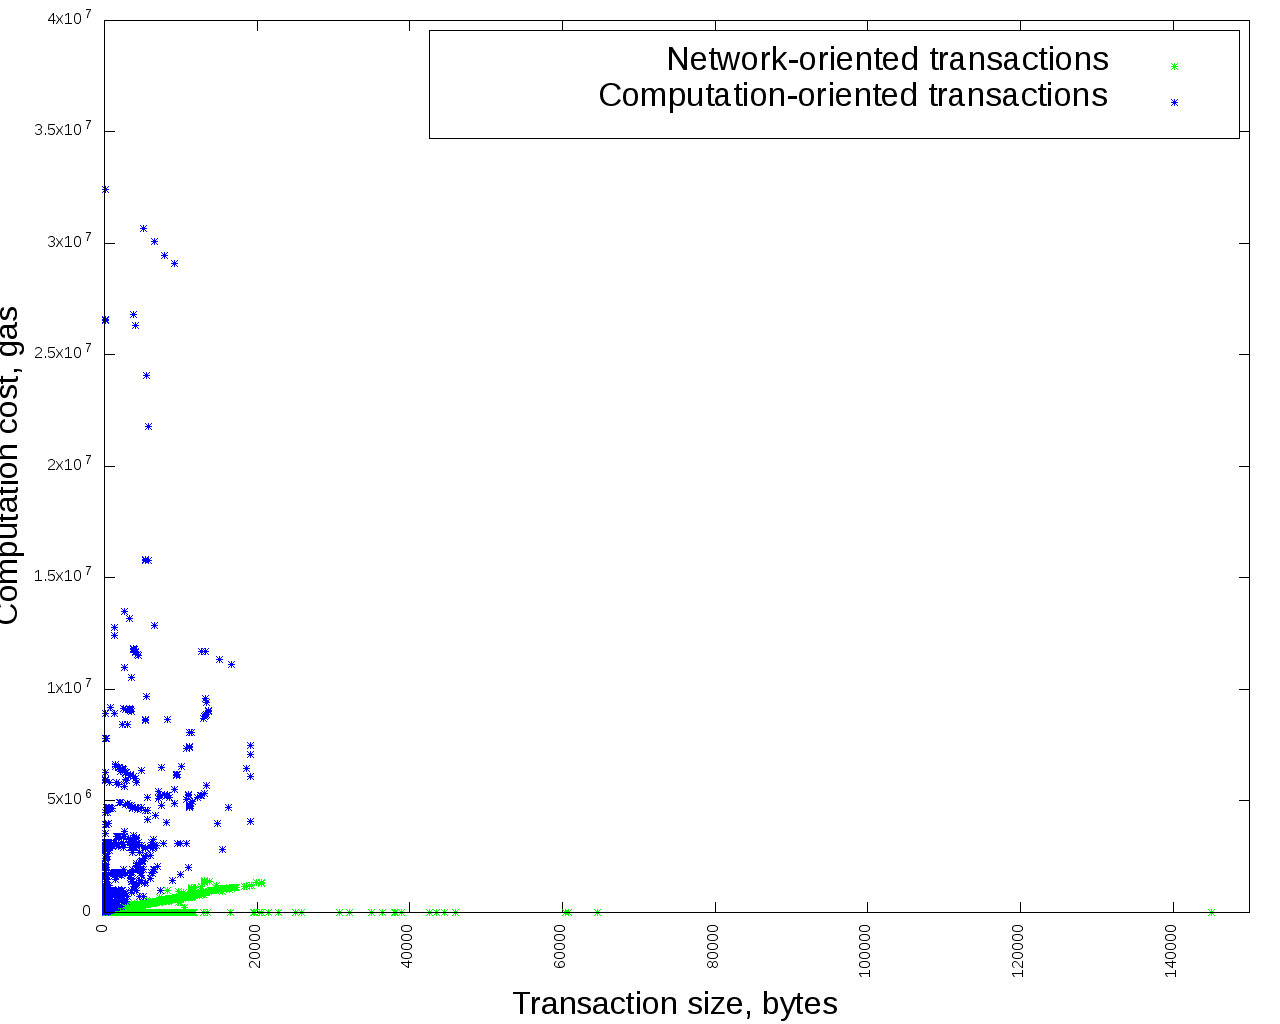
\includegraphics[width=\textwidth]{figures/txs-size-computation}
        \caption{}
        \label{fig:b}
    \end{subfigure}

    \begin{subfigure}[b]{0.48\textwidth}
        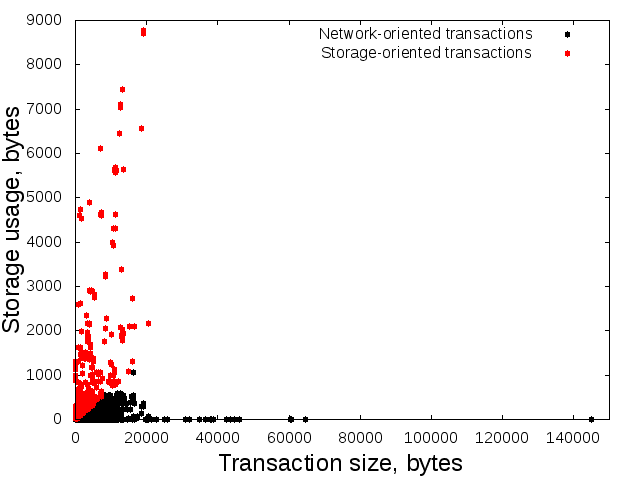
\includegraphics[width=\textwidth]{figures/txs-size-storage}
        \caption{}
        \label{fig:a}
    \end{subfigure}
    \begin{subfigure}[b]{0.48\textwidth}
        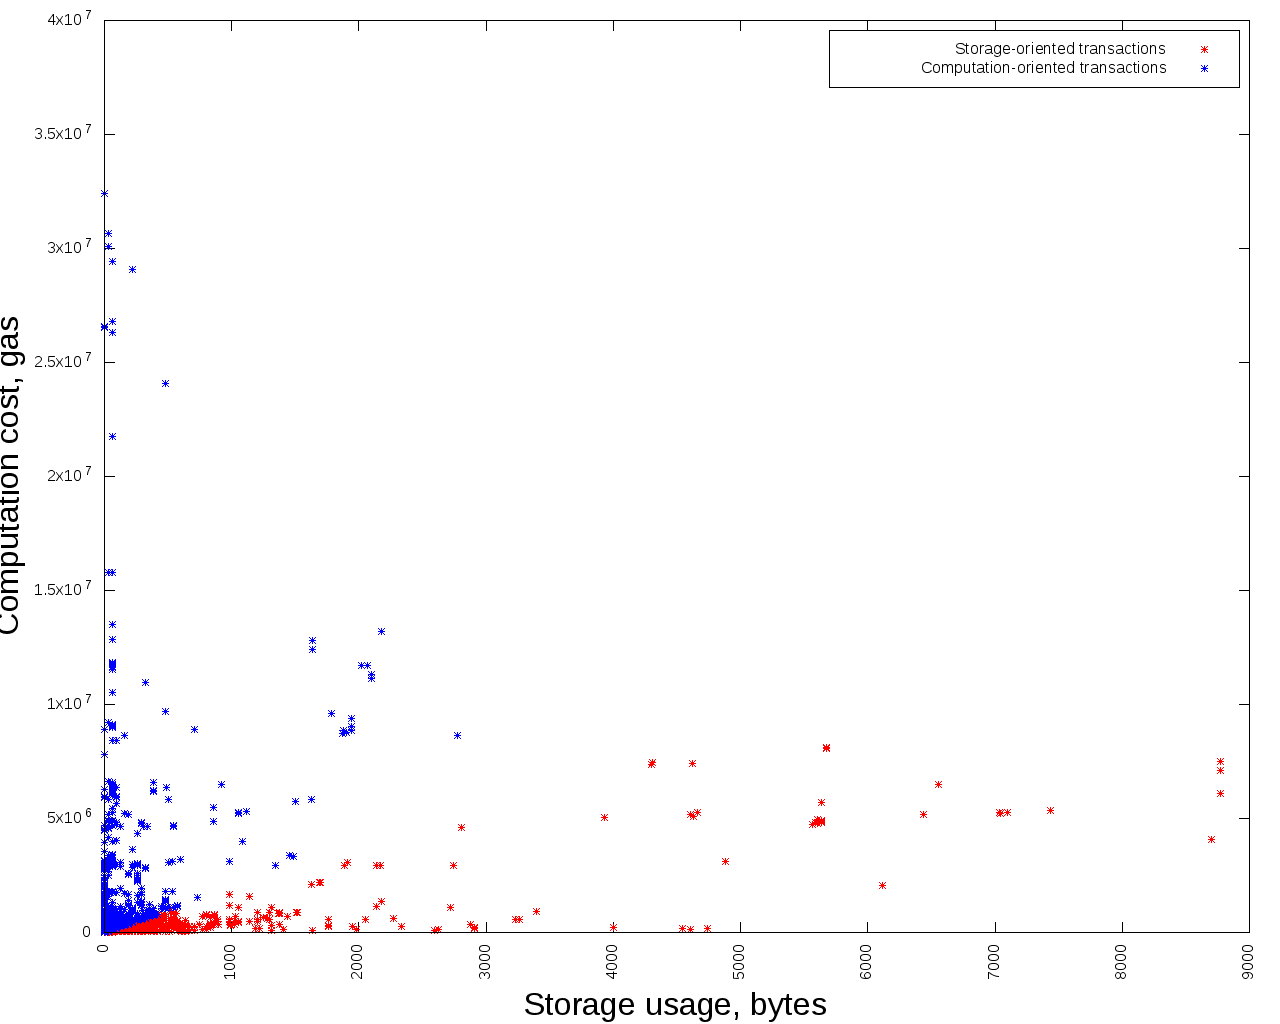
\includegraphics[width=\textwidth]{figures/txs-storage-computation}
        \caption{}
        \label{fig:b}
    \end{subfigure}

    \caption{Ethereum transactions differentiation by resource consumption}
    \label{fig:eth}
\end{figure}

The results of processing first $2\cdot10^6$ blocks in Ethereum network are presented in Figure~\ref{fig:eth}.
Each point corresponds to a transaction.
One can notice that parts of the distribution in Figure~\ref{fig:eth} extend
along the coordinate axis --- these are the transactions which can be
unambiguously distinguished by their type of the resource consumption. Their
presence confirms our expectations on the nature of resource consumption, and
serves as a justification of the proposed classification scheme. The space of
transactions is split into three parts by the aforementioned vector $\mathbf{n}$
with the endpoint at the first momentum of the transactions with at least 2
non-zero components, and thus not evident affiliation to a concrete type.

Another parameter of interest is the storage time. Using it directly
from the blockchain is weakly relevant to our scheme because the participants are not incentivized to remove data from the state earlier rather than later.
However, we consider the delay between the data submission and a first request to be the reliable parameter reflecting the needs of the users.
Analysis of Ethereum blockchain showed that in a lot of cases data stored in the state
was touched by other transactions in the same block or few blocks after insertion.
We filter out such cases as they do not show using blockchain as a storage. Excluding such short-lived data from our analysis
we estimate that average lifetime of a data object in Ethereum is 23,731 blocks~(or about 4 days
considering 15 seconds average delay between blocks).

This gives the following estimation on the ratio between the pricing coefficients for the expected state size:

\begin{align}
\begin{split}
&\frac{\alpha}{\beta} \approx 7.7\cdot10^{-3} \\
&\frac{\alpha}{S} \approx 6.7\cdot10^{-4}
\end{split}
\end{align}

where $S$ is the cost of the storage of byte of output in the state for one block, which does
not depend on state size in Ethereum. The estimations are quite approximate, while changing
them do not affect fees for most of transactions unambiguously attributed by a concrete type of the resource consumption.

\section{Discussion}
\label{sec:conslusion}

In the present work we addressed the problem of transaction fees in cryptocurrencies.
We proposed to devide fee into three parts depending on type of utilized resource:
network, computation or storage, and to charge only for a resource which
consumed at most, thus deviding transactions into three categories: network-oriented,
computation-oriented or storage-oriented. The analysis of Ethereum blockchain showed,
that the distribution of transactions in such 3-dimentional space extend along the
coordinate axis, allowing to unambiguously distinguish transactions by their
type of the resource consumption. This evinced self-consistency of our treatment,
and gave the reference parameters for possible implementation.

%that parts of the distribution in Figure~\ref{fig:eth} extend
% along the coordinate axis

The main attention was paid to calculation of storage fees. We argue that in
this fees should depend on space-time multiplication to make the state size
more predictable and it can be achieved even without rigid restriction on the
maximal state size. We proposed a concrete way to charge for state bytes consumed
that can be fully implemented on the script level.

Despite of the limitation of the state size growth, spacetime fees provides valuable side effects.
Due to structure of this fees, coins with lost keys returns into circulation with constant rate.
Although necessity of coin recirculation is still an open question, the need of lost coins recirculation
has been widely discussed in the literature (e.g. \cite{gjermundrod2014recirculating,gjermundrod2016going})
in regards with combat deflation that may eventually occur in cryptocurrencies with fixed supply and
was even implemented in some cryptocurrencies\cite{freicoin}.

Another important side effect of spacetime fee is that it provide static block reward
for miners. Even when a predetermined number of coins will enter a circulation,
spacetime fee will provide reward for miners, that does not depend on transaction
fees, preventing destructive but profitable mining strategies described in
~\cite{carlsten2016instability}.

With these factors taken into account, the ready-to-implement system is provided,
which is believed to slove the problem of uncontrollable state growth, provide some
valuable side effecrs by the same means, while preserving currently existing
methods for transaction fees and code execution costs.


%In the present work we addressed the problem of growth of the state size for the
%blockchain systems. Proposed solution --- spacetime fees --- relies on the
%economical factors rather than on solely the protocol itself. The idea of
%spacetime fees led us to the necessity of classification of the transactions by
%the type of resource consumption, and the simplest fee realization by
%$\max$-estimate caused the introduction of chain-based {\it scheduled payments}.
%It is shown that the described scheme can be fully implemented on the script
%level. The analysis of Ethereum blockchain evinced self-consistency of our
%treatment, and gave the reference parameters for possible implementation. We
%argue that the proposed solution makes the state size more predictable, which is
%crucial for decentrslization, and it can be achieved even without rigid
%restriction on the maximal state size. A valuable side effect of the spacetime
%fees is recirculation of the lost UTXOs in a long-run. With these factors taken
%into account, the ready-to-implement system is provided, which is believed to
%slove (at least partially) the problem of uncontrollable state growth, and
%recirculation of UTXOs by the same means, while preserving currently existing
%methods for transaction fees and code execution costs.

\bibliographystyle{splncs03}
\bibliography{sources.bib}

%\appendix
%
%\section{State size dynamics}
%\label{apx:statesize}
%For the primary analysis we assume that participants act honestly: they submit
%data if they need to do so and it is affordable; they do not in the opposite
%case. For the sake of simplicity, suppose that the time of storage of data
%block is fixed, and equal to $T$. In order to reduce the discrete stochastic
%model to continuous deterministic one, assume that the number of participants
%is large, and the typical size of the submitted data chunk is much less than
%characteristic pricing curve variation scale. The amount of data submitted to
%the state is changing continuously. At every given moment of time the users
%submit the data at some rate (say, MB/s) $f$, which is defined by the current
%price (participants submit more when cheap, and less when expensive). The
%current price is fully determined by the current state load $x$. After time
%interval $T$ data is erased from the state. The data is written into the state
%at rate $f(x(t))$, and erased at rate $f(x(t-T))$. Under these assumptions,
%the evolution of the state load is defined by the following equation:
%\begin{equation}
%    \frac{dx}{dt} = f(x(t))-f(x(t-T))\,.
%    \label{eq:dde0}
%\end{equation}
%If one measures time in the data block TTL $T$, the equation takes the form
%\begin{equation}
%    \dot{x} = f(x(t))-f(x(t-1))\,.
%    \label{eq:dde1}
%\end{equation}
%The equations of this type are called delay differential equations (DDE), and have
%been studied widely for the vast amount of control problems.
%
%Now few words about the function $f$, and how to convert it to the miner's
%income. What participants know is the pricing curve $S(x)$. For every value $P$
%of this function there is amount of people $N(S)$ who want to submit data and
%can afford it at time interval $T$. The function $N(S)$ is non-increasing, and
%going to zero for sufficiently large $S$ (every participant has maximal price he
%is ready to pay, and will also try to submit something if current price is
%lower; for sufficiently large price no one is ready to pay). In these notations
%$f(x)=N(S(x))$ (see inset on Figure~\ref{fig:rewards}), and the profit rate which
%miners get from current submissions is $y(t) = S(x(t))f(x(t))$.
%
%\subsection{Constant storage price}
%\subsection{State-dependent storage price}
%\begin{figure}
%    \includestandalone[width=\textwidth]{figures/dynamics}
%    \caption{
%        \label{fig:dynamics} Dynamics of the state size for various initial
%        rates. The numbers above the curves are the miners reward rates with
%        respect to maximal possible stationary rewards.
%    }
%\end{figure}

\end{document}
